%% Anonymised manuscript for double-blind review (Neural Computing and Applications).
%% Author names, affiliations, acknowledgements and funding are on the separate
%% title page (title_page.tex).
%% Every reported result is a \val{...} lookup generated from the stored
%% evaluation files by analysis/make_tables.py (see generated/numbers.tex).
\documentclass[pdflatex,iicol,sn-basic,Numbered]{sn-jnl}

\usepackage{graphicx}%
\usepackage{amsmath,amssymb,amsfonts}%
\usepackage{xcolor}%
\usepackage{textcomp}%
\usepackage{booktabs}%
\usepackage{multirow}%
\usepackage{pgfplots}%
\pgfplotsset{compat=1.18}%
\usepgfplotslibrary{groupplots}%
\usetikzlibrary{positioning,arrows.meta,fit,calc,backgrounds,patterns,shapes.geometric}%

% Generated by latex_project/analysis/make_tables.py - do not edit.
\makeatletter
\newcommand{\val}[1]{\ifcsname val@#1\endcsname\csname val@#1\endcsname\else\textbf{\textcolor{red}{??#1}}\PackageWarning{numbers}{Undefined value #1}\fi}
\newcommand{\hasval}[1]{\ifcsname val@#1\endcsname\expandafter\@firstoftwo\else\expandafter\@secondoftwo\fi}
\expandafter\def\csname val@a.cyc-detr.ap\endcsname{1.50}
\expandafter\def\csname val@a.cyc-detr.ap50\endcsname{1.24}
\expandafter\def\csname val@a.cyc-detr.ap55\endcsname{1.62}
\expandafter\def\csname val@a.cyc-detr.ap60\endcsname{1.77}
\expandafter\def\csname val@a.cyc-detr.ap65\endcsname{1.36}
\expandafter\def\csname val@a.cyc-detr.ap70\endcsname{1.87}
\expandafter\def\csname val@a.cyc-detr.ap75\endcsname{1.40}
\expandafter\def\csname val@a.cyc-detr.ap80\endcsname{1.32}
\expandafter\def\csname val@a.cyc-detr.ap85\endcsname{1.97}
\expandafter\def\csname val@a.cyc-detr.ap90\endcsname{1.59}
\expandafter\def\csname val@a.cyc-detr.ap95\endcsname{0.85}
\expandafter\def\csname val@a.cyc-detr.ioumaxabs\endcsname{1.97}
\expandafter\def\csname val@a.cyc-detr.iouminabs\endcsname{0.85}
\expandafter\def\csname val@a.cyc-detr.midmax\endcsname{1.32}
\expandafter\def\csname val@a.cyc-detr.midmin\endcsname{1.97}
\expandafter\def\csname val@a.rt23-rt2.ap\endcsname{1.29}
\expandafter\def\csname val@a.rt23-rt2.ap50\endcsname{1.07}
\expandafter\def\csname val@a.rt23-rt2.ap55\endcsname{1.23}
\expandafter\def\csname val@a.rt23-rt2.ap60\endcsname{1.30}
\expandafter\def\csname val@a.rt23-rt2.ap65\endcsname{1.18}
\expandafter\def\csname val@a.rt23-rt2.ap70\endcsname{1.34}
\expandafter\def\csname val@a.rt23-rt2.ap75\endcsname{1.11}
\expandafter\def\csname val@a.rt23-rt2.ap80\endcsname{1.65}
\expandafter\def\csname val@a.rt23-rt2.ap85\endcsname{1.88}
\expandafter\def\csname val@a.rt23-rt2.ap90\endcsname{1.32}
\expandafter\def\csname val@a.rt23-rt2.ap95\endcsname{0.86}
\expandafter\def\csname val@a.rt23-rt2.ioumaxabs\endcsname{1.88}
\expandafter\def\csname val@a.rt23-rt2.iouminabs\endcsname{0.86}
\expandafter\def\csname val@a.rt23-rt2.midmax\endcsname{1.88}
\expandafter\def\csname val@a.rt23-rt2.midmin\endcsname{1.11}
\expandafter\def\csname val@a.rt23-rt6.ap\endcsname{0.71}
\expandafter\def\csname val@a.rt23-rt6.ap50\endcsname{0.25}
\expandafter\def\csname val@a.rt23-rt6.ap55\endcsname{0.50}
\expandafter\def\csname val@a.rt23-rt6.ap60\endcsname{0.67}
\expandafter\def\csname val@a.rt23-rt6.ap65\endcsname{0.82}
\expandafter\def\csname val@a.rt23-rt6.ap70\endcsname{0.97}
\expandafter\def\csname val@a.rt23-rt6.ap75\endcsname{1.27}
\expandafter\def\csname val@a.rt23-rt6.ap80\endcsname{1.61}
\expandafter\def\csname val@a.rt23-rt6.ap85\endcsname{1.31}
\expandafter\def\csname val@a.rt23-rt6.ap90\endcsname{0.63}
\expandafter\def\csname val@a.rt23-rt6.ap95\endcsname{0.87}
\expandafter\def\csname val@a.rt23-rt6.ioumaxabs\endcsname{1.61}
\expandafter\def\csname val@a.rt23-rt6.iouminabs\endcsname{0.25}
\expandafter\def\csname val@a.rt23-rt6.midmax\endcsname{1.61}
\expandafter\def\csname val@a.rt23-rt6.midmin\endcsname{0.97}
\expandafter\def\csname val@a.rt32-rt2.ap\endcsname{1.36}
\expandafter\def\csname val@a.rt32-rt2.ap50\endcsname{0.60}
\expandafter\def\csname val@a.rt32-rt2.ap55\endcsname{0.93}
\expandafter\def\csname val@a.rt32-rt2.ap60\endcsname{1.09}
\expandafter\def\csname val@a.rt32-rt2.ap65\endcsname{1.21}
\expandafter\def\csname val@a.rt32-rt2.ap70\endcsname{1.28}
\expandafter\def\csname val@a.rt32-rt2.ap75\endcsname{1.32}
\expandafter\def\csname val@a.rt32-rt2.ap80\endcsname{2.12}
\expandafter\def\csname val@a.rt32-rt2.ap85\endcsname{2.37}
\expandafter\def\csname val@a.rt32-rt2.ap90\endcsname{1.79}
\expandafter\def\csname val@a.rt32-rt2.ap95\endcsname{0.90}
\expandafter\def\csname val@a.rt32-rt2.ioumaxabs\endcsname{2.37}
\expandafter\def\csname val@a.rt32-rt2.iouminabs\endcsname{0.60}
\expandafter\def\csname val@a.rt32-rt2.midmax\endcsname{2.37}
\expandafter\def\csname val@a.rt32-rt2.midmin\endcsname{1.28}
\expandafter\def\csname val@a.rt32-rt6.ap\endcsname{0.78}
\expandafter\def\csname val@a.rt32-rt6.ap50\endcsname{0.23}
\expandafter\def\csname val@a.rt32-rt6.ap55\endcsname{0.20}
\expandafter\def\csname val@a.rt32-rt6.ap60\endcsname{0.46}
\expandafter\def\csname val@a.rt32-rt6.ap65\endcsname{0.85}
\expandafter\def\csname val@a.rt32-rt6.ap70\endcsname{0.91}
\expandafter\def\csname val@a.rt32-rt6.ap75\endcsname{1.48}
\expandafter\def\csname val@a.rt32-rt6.ap80\endcsname{2.08}
\expandafter\def\csname val@a.rt32-rt6.ap85\endcsname{1.80}
\expandafter\def\csname val@a.rt32-rt6.ap90\endcsname{1.10}
\expandafter\def\csname val@a.rt32-rt6.ap95\endcsname{0.83}
\expandafter\def\csname val@a.rt32-rt6.ioumaxabs\endcsname{2.08}
\expandafter\def\csname val@a.rt32-rt6.iouminabs\endcsname{0.20}
\expandafter\def\csname val@a.rt32-rt6.midmax\endcsname{2.08}
\expandafter\def\csname val@a.rt32-rt6.midmin\endcsname{0.91}
\expandafter\def\csname val@a.rt6-rt2.ap\endcsname{0.58}
\expandafter\def\csname val@a.rt6-rt2.ap50\endcsname{0.82}
\expandafter\def\csname val@a.rt6-rt2.ap55\endcsname{0.73}
\expandafter\def\csname val@a.rt6-rt2.ap60\endcsname{0.63}
\expandafter\def\csname val@a.rt6-rt2.ap65\endcsname{0.36}
\expandafter\def\csname val@a.rt6-rt2.ap70\endcsname{0.37}
\expandafter\def\csname val@a.rt6-rt2.ap75\endcsname{0.16}
\expandafter\def\csname val@a.rt6-rt2.ap80\endcsname{0.03}
\expandafter\def\csname val@a.rt6-rt2.ap85\endcsname{0.57}
\expandafter\def\csname val@a.rt6-rt2.ap90\endcsname{0.69}
\expandafter\def\csname val@a.rt6-rt2.ap95\endcsname{1.73}
\expandafter\def\csname val@a.rt6-rt2.ioumaxabs\endcsname{1.73}
\expandafter\def\csname val@a.rt6-rt2.iouminabs\endcsname{0.03}
\expandafter\def\csname val@a.rt6-rt2.midmax\endcsname{0.57}
\expandafter\def\csname val@a.rt6-rt2.midmin\endcsname{0.16}
\expandafter\def\csname val@a.seq-detr.ap\endcsname{4.07}
\expandafter\def\csname val@a.seq-detr.ap50\endcsname{4.29}
\expandafter\def\csname val@a.seq-detr.ap55\endcsname{4.48}
\expandafter\def\csname val@a.seq-detr.ap60\endcsname{4.56}
\expandafter\def\csname val@a.seq-detr.ap65\endcsname{4.50}
\expandafter\def\csname val@a.seq-detr.ap70\endcsname{5.20}
\expandafter\def\csname val@a.seq-detr.ap75\endcsname{4.84}
\expandafter\def\csname val@a.seq-detr.ap80\endcsname{4.70}
\expandafter\def\csname val@a.seq-detr.ap85\endcsname{4.29}
\expandafter\def\csname val@a.seq-detr.ap90\endcsname{2.68}
\expandafter\def\csname val@a.seq-detr.ap95\endcsname{1.15}
\expandafter\def\csname val@a.seq-detr.ioumaxabs\endcsname{5.20}
\expandafter\def\csname val@a.seq-detr.iouminabs\endcsname{1.15}
\expandafter\def\csname val@a.seq-detr.midmax\endcsname{4.29}
\expandafter\def\csname val@a.seq-detr.midmin\endcsname{5.20}
\expandafter\def\csname val@cyc.ap\endcsname{45.69}
\expandafter\def\csname val@cyc.ap50\endcsname{73.03}
\expandafter\def\csname val@cyc.ap55\endcsname{69.69}
\expandafter\def\csname val@cyc.ap60\endcsname{65.69}
\expandafter\def\csname val@cyc.ap65\endcsname{61.06}
\expandafter\def\csname val@cyc.ap70\endcsname{54.70}
\expandafter\def\csname val@cyc.ap75\endcsname{47.80}
\expandafter\def\csname val@cyc.ap80\endcsname{39.03}
\expandafter\def\csname val@cyc.ap85\endcsname{27.85}
\expandafter\def\csname val@cyc.ap90\endcsname{15.13}
\expandafter\def\csname val@cyc.ap95\endcsname{2.88}
\expandafter\def\csname val@cyc.decgflops\endcsname{1.33}
\expandafter\def\csname val@cyc.encgflops\endcsname{7.12}
\expandafter\def\csname val@cyc.gflops\endcsname{68.4}
\expandafter\def\csname val@cyc.params\endcsname{33.12}
\expandafter\def\csname val@cyc.routers\endcsname{1028}
\expandafter\def\csname val@cyc.tfgflops\endcsname{8.45}
\expandafter\def\csname val@cyc.tfgflopsred\endcsname{25}
\expandafter\def\csname val@cyc.tfparams\endcsname{11.58}
\expandafter\def\csname val@cyc.trainable\endcsname{11.85}
\expandafter\def\csname val@cyc.trainred\endcsname{49}
\expandafter\def\csname val@d.cyc-detr.ap\endcsname{\textminus 1.50}
\expandafter\def\csname val@d.cyc-detr.ap50\endcsname{\textminus 1.24}
\expandafter\def\csname val@d.cyc-detr.ap55\endcsname{\textminus 1.62}
\expandafter\def\csname val@d.cyc-detr.ap60\endcsname{\textminus 1.77}
\expandafter\def\csname val@d.cyc-detr.ap65\endcsname{\textminus 1.36}
\expandafter\def\csname val@d.cyc-detr.ap70\endcsname{\textminus 1.87}
\expandafter\def\csname val@d.cyc-detr.ap75\endcsname{\textminus 1.40}
\expandafter\def\csname val@d.cyc-detr.ap80\endcsname{\textminus 1.32}
\expandafter\def\csname val@d.cyc-detr.ap85\endcsname{\textminus 1.97}
\expandafter\def\csname val@d.cyc-detr.ap90\endcsname{\textminus 1.59}
\expandafter\def\csname val@d.cyc-detr.ap95\endcsname{\textminus 0.85}
\expandafter\def\csname val@d.cyc-detr.ioumaxabs\endcsname{1.97}
\expandafter\def\csname val@d.cyc-detr.iouminabs\endcsname{0.85}
\expandafter\def\csname val@d.cyc-detr.midmax\endcsname{\textminus 1.32}
\expandafter\def\csname val@d.cyc-detr.midmin\endcsname{\textminus 1.97}
\expandafter\def\csname val@d.rt23-rt2.ap\endcsname{+1.29}
\expandafter\def\csname val@d.rt23-rt2.ap50\endcsname{+1.07}
\expandafter\def\csname val@d.rt23-rt2.ap55\endcsname{+1.23}
\expandafter\def\csname val@d.rt23-rt2.ap60\endcsname{+1.30}
\expandafter\def\csname val@d.rt23-rt2.ap65\endcsname{+1.18}
\expandafter\def\csname val@d.rt23-rt2.ap70\endcsname{+1.34}
\expandafter\def\csname val@d.rt23-rt2.ap75\endcsname{+1.11}
\expandafter\def\csname val@d.rt23-rt2.ap80\endcsname{+1.65}
\expandafter\def\csname val@d.rt23-rt2.ap85\endcsname{+1.88}
\expandafter\def\csname val@d.rt23-rt2.ap90\endcsname{+1.32}
\expandafter\def\csname val@d.rt23-rt2.ap95\endcsname{+0.86}
\expandafter\def\csname val@d.rt23-rt2.ioumaxabs\endcsname{1.88}
\expandafter\def\csname val@d.rt23-rt2.iouminabs\endcsname{0.86}
\expandafter\def\csname val@d.rt23-rt2.midmax\endcsname{+1.88}
\expandafter\def\csname val@d.rt23-rt2.midmin\endcsname{+1.11}
\expandafter\def\csname val@d.rt23-rt6.ap\endcsname{+0.71}
\expandafter\def\csname val@d.rt23-rt6.ap50\endcsname{+0.25}
\expandafter\def\csname val@d.rt23-rt6.ap55\endcsname{+0.50}
\expandafter\def\csname val@d.rt23-rt6.ap60\endcsname{+0.67}
\expandafter\def\csname val@d.rt23-rt6.ap65\endcsname{+0.82}
\expandafter\def\csname val@d.rt23-rt6.ap70\endcsname{+0.97}
\expandafter\def\csname val@d.rt23-rt6.ap75\endcsname{+1.27}
\expandafter\def\csname val@d.rt23-rt6.ap80\endcsname{+1.61}
\expandafter\def\csname val@d.rt23-rt6.ap85\endcsname{+1.31}
\expandafter\def\csname val@d.rt23-rt6.ap90\endcsname{+0.63}
\expandafter\def\csname val@d.rt23-rt6.ap95\endcsname{\textminus 0.87}
\expandafter\def\csname val@d.rt23-rt6.ioumaxabs\endcsname{1.61}
\expandafter\def\csname val@d.rt23-rt6.iouminabs\endcsname{0.25}
\expandafter\def\csname val@d.rt23-rt6.midmax\endcsname{+1.61}
\expandafter\def\csname val@d.rt23-rt6.midmin\endcsname{+0.97}
\expandafter\def\csname val@d.rt32-rt2.ap\endcsname{+1.36}
\expandafter\def\csname val@d.rt32-rt2.ap50\endcsname{+0.60}
\expandafter\def\csname val@d.rt32-rt2.ap55\endcsname{+0.93}
\expandafter\def\csname val@d.rt32-rt2.ap60\endcsname{+1.09}
\expandafter\def\csname val@d.rt32-rt2.ap65\endcsname{+1.21}
\expandafter\def\csname val@d.rt32-rt2.ap70\endcsname{+1.28}
\expandafter\def\csname val@d.rt32-rt2.ap75\endcsname{+1.32}
\expandafter\def\csname val@d.rt32-rt2.ap80\endcsname{+2.12}
\expandafter\def\csname val@d.rt32-rt2.ap85\endcsname{+2.37}
\expandafter\def\csname val@d.rt32-rt2.ap90\endcsname{+1.79}
\expandafter\def\csname val@d.rt32-rt2.ap95\endcsname{+0.90}
\expandafter\def\csname val@d.rt32-rt2.ioumaxabs\endcsname{2.37}
\expandafter\def\csname val@d.rt32-rt2.iouminabs\endcsname{0.60}
\expandafter\def\csname val@d.rt32-rt2.midmax\endcsname{+2.37}
\expandafter\def\csname val@d.rt32-rt2.midmin\endcsname{+1.28}
\expandafter\def\csname val@d.rt32-rt6.ap\endcsname{+0.78}
\expandafter\def\csname val@d.rt32-rt6.ap50\endcsname{\textminus 0.23}
\expandafter\def\csname val@d.rt32-rt6.ap55\endcsname{+0.20}
\expandafter\def\csname val@d.rt32-rt6.ap60\endcsname{+0.46}
\expandafter\def\csname val@d.rt32-rt6.ap65\endcsname{+0.85}
\expandafter\def\csname val@d.rt32-rt6.ap70\endcsname{+0.91}
\expandafter\def\csname val@d.rt32-rt6.ap75\endcsname{+1.48}
\expandafter\def\csname val@d.rt32-rt6.ap80\endcsname{+2.08}
\expandafter\def\csname val@d.rt32-rt6.ap85\endcsname{+1.80}
\expandafter\def\csname val@d.rt32-rt6.ap90\endcsname{+1.10}
\expandafter\def\csname val@d.rt32-rt6.ap95\endcsname{\textminus 0.83}
\expandafter\def\csname val@d.rt32-rt6.ioumaxabs\endcsname{2.08}
\expandafter\def\csname val@d.rt32-rt6.iouminabs\endcsname{0.20}
\expandafter\def\csname val@d.rt32-rt6.midmax\endcsname{+2.08}
\expandafter\def\csname val@d.rt32-rt6.midmin\endcsname{+0.91}
\expandafter\def\csname val@d.rt6-rt2.ap\endcsname{+0.58}
\expandafter\def\csname val@d.rt6-rt2.ap50\endcsname{+0.82}
\expandafter\def\csname val@d.rt6-rt2.ap55\endcsname{+0.73}
\expandafter\def\csname val@d.rt6-rt2.ap60\endcsname{+0.63}
\expandafter\def\csname val@d.rt6-rt2.ap65\endcsname{+0.36}
\expandafter\def\csname val@d.rt6-rt2.ap70\endcsname{+0.37}
\expandafter\def\csname val@d.rt6-rt2.ap75\endcsname{\textminus 0.16}
\expandafter\def\csname val@d.rt6-rt2.ap80\endcsname{+0.03}
\expandafter\def\csname val@d.rt6-rt2.ap85\endcsname{+0.57}
\expandafter\def\csname val@d.rt6-rt2.ap90\endcsname{+0.69}
\expandafter\def\csname val@d.rt6-rt2.ap95\endcsname{+1.73}
\expandafter\def\csname val@d.rt6-rt2.ioumaxabs\endcsname{1.73}
\expandafter\def\csname val@d.rt6-rt2.iouminabs\endcsname{0.03}
\expandafter\def\csname val@d.rt6-rt2.midmax\endcsname{+0.57}
\expandafter\def\csname val@d.rt6-rt2.midmin\endcsname{\textminus 0.16}
\expandafter\def\csname val@d.seq-detr.ap\endcsname{\textminus 4.07}
\expandafter\def\csname val@d.seq-detr.ap50\endcsname{\textminus 4.29}
\expandafter\def\csname val@d.seq-detr.ap55\endcsname{\textminus 4.48}
\expandafter\def\csname val@d.seq-detr.ap60\endcsname{\textminus 4.56}
\expandafter\def\csname val@d.seq-detr.ap65\endcsname{\textminus 4.50}
\expandafter\def\csname val@d.seq-detr.ap70\endcsname{\textminus 5.20}
\expandafter\def\csname val@d.seq-detr.ap75\endcsname{\textminus 4.84}
\expandafter\def\csname val@d.seq-detr.ap80\endcsname{\textminus 4.70}
\expandafter\def\csname val@d.seq-detr.ap85\endcsname{\textminus 4.29}
\expandafter\def\csname val@d.seq-detr.ap90\endcsname{\textminus 2.68}
\expandafter\def\csname val@d.seq-detr.ap95\endcsname{\textminus 1.15}
\expandafter\def\csname val@d.seq-detr.ioumaxabs\endcsname{5.20}
\expandafter\def\csname val@d.seq-detr.iouminabs\endcsname{1.15}
\expandafter\def\csname val@d.seq-detr.midmax\endcsname{\textminus 4.29}
\expandafter\def\csname val@d.seq-detr.midmin\endcsname{\textminus 5.20}
\expandafter\def\csname val@depth.cyc.1.iou\endcsname{0.80}
\expandafter\def\csname val@depth.cyc.1.iou75\endcsname{73}
\expandafter\def\csname val@depth.cyc.1.objs\endcsname{4.1}
\expandafter\def\csname val@depth.cyc.1.prob\endcsname{0.88}
\expandafter\def\csname val@depth.cyc.1.share\endcsname{75}
\expandafter\def\csname val@depth.cyc.2.iou\endcsname{0.60}
\expandafter\def\csname val@depth.cyc.2.iou75\endcsname{30}
\expandafter\def\csname val@depth.cyc.2.objs\endcsname{7.3}
\expandafter\def\csname val@depth.cyc.2.prob\endcsname{0.62}
\expandafter\def\csname val@depth.cyc.2.share\endcsname{13}
\expandafter\def\csname val@depth.cyc.3.iou\endcsname{0.57}
\expandafter\def\csname val@depth.cyc.3.iou75\endcsname{23}
\expandafter\def\csname val@depth.cyc.3.objs\endcsname{7.9}
\expandafter\def\csname val@depth.cyc.3.prob\endcsname{0.60}
\expandafter\def\csname val@depth.cyc.3.share\endcsname{12}
\expandafter\def\csname val@depth.rt23.1.iou\endcsname{0.84}
\expandafter\def\csname val@depth.rt23.1.iou75\endcsname{82}
\expandafter\def\csname val@depth.rt23.1.objs\endcsname{4.5}
\expandafter\def\csname val@depth.rt23.1.prob\endcsname{0.83}
\expandafter\def\csname val@depth.rt23.1.share\endcsname{63}
\expandafter\def\csname val@depth.rt23.2.iou\endcsname{0.84}
\expandafter\def\csname val@depth.rt23.2.iou75\endcsname{80}
\expandafter\def\csname val@depth.rt23.2.objs\endcsname{5.3}
\expandafter\def\csname val@depth.rt23.2.prob\endcsname{0.77}
\expandafter\def\csname val@depth.rt23.2.share\endcsname{30}
\expandafter\def\csname val@depth.rt23.3.iou\endcsname{0.76}
\expandafter\def\csname val@depth.rt23.3.iou75\endcsname{65}
\expandafter\def\csname val@depth.rt23.3.objs\endcsname{7.7}
\expandafter\def\csname val@depth.rt23.3.prob\endcsname{0.62}
\expandafter\def\csname val@depth.rt23.3.share\endcsname{7}
\expandafter\def\csname val@depth.rt32.1.iou\endcsname{0.83}
\expandafter\def\csname val@depth.rt32.1.iou75\endcsname{78}
\expandafter\def\csname val@depth.rt32.1.objs\endcsname{4.8}
\expandafter\def\csname val@depth.rt32.1.prob\endcsname{0.79}
\expandafter\def\csname val@depth.rt32.1.share\endcsname{56}
\expandafter\def\csname val@depth.rt32.2.iou\endcsname{0.85}
\expandafter\def\csname val@depth.rt32.2.iou75\endcsname{82}
\expandafter\def\csname val@depth.rt32.2.objs\endcsname{5.1}
\expandafter\def\csname val@depth.rt32.2.prob\endcsname{0.79}
\expandafter\def\csname val@depth.rt32.2.share\endcsname{44}
\expandafter\def\csname val@depth.seq.1.iou\endcsname{0.81}
\expandafter\def\csname val@depth.seq.1.iou75\endcsname{76}
\expandafter\def\csname val@depth.seq.1.objs\endcsname{3.6}
\expandafter\def\csname val@depth.seq.1.prob\endcsname{0.90}
\expandafter\def\csname val@depth.seq.1.share\endcsname{62}
\expandafter\def\csname val@depth.seq.2.iou\endcsname{0.66}
\expandafter\def\csname val@depth.seq.2.iou75\endcsname{40}
\expandafter\def\csname val@depth.seq.2.objs\endcsname{6.5}
\expandafter\def\csname val@depth.seq.2.prob\endcsname{0.71}
\expandafter\def\csname val@depth.seq.2.share\endcsname{8}
\expandafter\def\csname val@depth.seq.3.iou\endcsname{0.65}
\expandafter\def\csname val@depth.seq.3.iou75\endcsname{38}
\expandafter\def\csname val@depth.seq.3.objs\endcsname{6.8}
\expandafter\def\csname val@depth.seq.3.prob\endcsname{0.66}
\expandafter\def\csname val@depth.seq.3.share\endcsname{10}
\expandafter\def\csname val@depth.seq.4.iou\endcsname{0.56}
\expandafter\def\csname val@depth.seq.4.iou75\endcsname{20}
\expandafter\def\csname val@depth.seq.4.objs\endcsname{7.5}
\expandafter\def\csname val@depth.seq.4.prob\endcsname{0.62}
\expandafter\def\csname val@depth.seq.4.share\endcsname{7}
\expandafter\def\csname val@depth.seq.5.iou\endcsname{0.59}
\expandafter\def\csname val@depth.seq.5.iou75\endcsname{27}
\expandafter\def\csname val@depth.seq.5.objs\endcsname{7.7}
\expandafter\def\csname val@depth.seq.5.prob\endcsname{0.63}
\expandafter\def\csname val@depth.seq.5.share\endcsname{7}
\expandafter\def\csname val@depth.seq.6.iou\endcsname{0.57}
\expandafter\def\csname val@depth.seq.6.iou75\endcsname{22}
\expandafter\def\csname val@depth.seq.6.objs\endcsname{7.5}
\expandafter\def\csname val@depth.seq.6.prob\endcsname{0.54}
\expandafter\def\csname val@depth.seq.6.share\endcsname{5}
\expandafter\def\csname val@detr.ap\endcsname{47.18}
\expandafter\def\csname val@detr.ap50\endcsname{74.27}
\expandafter\def\csname val@detr.ap55\endcsname{71.31}
\expandafter\def\csname val@detr.ap60\endcsname{67.46}
\expandafter\def\csname val@detr.ap65\endcsname{62.42}
\expandafter\def\csname val@detr.ap70\endcsname{56.56}
\expandafter\def\csname val@detr.ap75\endcsname{49.20}
\expandafter\def\csname val@detr.ap80\endcsname{40.35}
\expandafter\def\csname val@detr.ap85\endcsname{29.82}
\expandafter\def\csname val@detr.ap90\endcsname{16.73}
\expandafter\def\csname val@detr.ap95\endcsname{3.73}
\expandafter\def\csname val@detr.decgflops\endcsname{1.50}
\expandafter\def\csname val@detr.encgflops\endcsname{9.70}
\expandafter\def\csname val@detr.gflops\endcsname{71.2}
\expandafter\def\csname val@detr.params\endcsname{44.70}
\expandafter\def\csname val@detr.routers\endcsname{0}
\expandafter\def\csname val@detr.tfgflops\endcsname{11.20}
\expandafter\def\csname val@detr.tfparams\endcsname{23.15}
\expandafter\def\csname val@detr.trainable\endcsname{23.43}
\expandafter\def\csname val@fg.cyc.1.bg\endcsname{52}
\expandafter\def\csname val@fg.cyc.1.cap\endcsname{67}
\expandafter\def\csname val@fg.cyc.1.fg\endcsname{84}
\expandafter\def\csname val@fg.cyc.1.ratio\endcsname{1.61}
\expandafter\def\csname val@fg.cyc.2.bg\endcsname{17}
\expandafter\def\csname val@fg.cyc.2.cap\endcsname{33}
\expandafter\def\csname val@fg.cyc.2.fg\endcsname{53}
\expandafter\def\csname val@fg.cyc.2.ratio\endcsname{3.14}
\expandafter\def\csname val@fg.cyc.max\endcsname{3.14}
\expandafter\def\csname val@fg.cyc.min\endcsname{1.61}
\expandafter\def\csname val@fg.seq.1.bg\endcsname{84}
\expandafter\def\csname val@fg.seq.1.cap\endcsname{83}
\expandafter\def\csname val@fg.seq.1.fg\endcsname{83}
\expandafter\def\csname val@fg.seq.1.ratio\endcsname{0.99}
\expandafter\def\csname val@fg.seq.2.bg\endcsname{77}
\expandafter\def\csname val@fg.seq.2.cap\endcsname{67}
\expandafter\def\csname val@fg.seq.2.fg\endcsname{54}
\expandafter\def\csname val@fg.seq.2.ratio\endcsname{0.71}
\expandafter\def\csname val@fg.seq.3.bg\endcsname{53}
\expandafter\def\csname val@fg.seq.3.cap\endcsname{50}
\expandafter\def\csname val@fg.seq.3.fg\endcsname{47}
\expandafter\def\csname val@fg.seq.3.ratio\endcsname{0.89}
\expandafter\def\csname val@fg.seq.4.bg\endcsname{32}
\expandafter\def\csname val@fg.seq.4.cap\endcsname{33}
\expandafter\def\csname val@fg.seq.4.fg\endcsname{35}
\expandafter\def\csname val@fg.seq.4.ratio\endcsname{1.08}
\expandafter\def\csname val@fg.seq.5.bg\endcsname{14}
\expandafter\def\csname val@fg.seq.5.cap\endcsname{17}
\expandafter\def\csname val@fg.seq.5.fg\endcsname{20}
\expandafter\def\csname val@fg.seq.5.ratio\endcsname{1.42}
\expandafter\def\csname val@fg.seq.max\endcsname{1.42}
\expandafter\def\csname val@fg.seq.min\endcsname{0.71}
\expandafter\def\csname val@loss.cyc-detr\endcsname{18}
\expandafter\def\csname val@loss.rt23-rt2\endcsname{1}
\expandafter\def\csname val@loss.rt23-rt6\endcsname{4}
\expandafter\def\csname val@loss.rt32-rt2\endcsname{1}
\expandafter\def\csname val@loss.rt32-rt6\endcsname{4}
\expandafter\def\csname val@loss.rt6-rt2\endcsname{6}
\expandafter\def\csname val@loss.seq-detr\endcsname{20}
\expandafter\def\csname val@nclasses\endcsname{20}
\expandafter\def\csname val@probe.cyc.capacity\endcsname{25\textrightarrow{}16\textrightarrow{}8}
\expandafter\def\csname val@probe.cyc.default\endcsname{47.70}
\expandafter\def\csname val@probe.cyc.full\endcsname{\textminus 0.19}
\expandafter\def\csname val@probe.cyc.fulldecoder\endcsname{\textminus 0.05}
\expandafter\def\csname val@probe.cyc.fullencoder\endcsname{\textminus 0.04}
\expandafter\def\csname val@probe.cyc.maxabs\endcsname{0.62}
\expandafter\def\csname val@probe.cyc.nobj\endcsname{2{,}924}
\expandafter\def\csname val@probe.cyc.oracle\endcsname{\textminus 0.36}
\expandafter\def\csname val@probe.cyc.random\endcsname{\textminus 0.62}
\expandafter\def\csname val@probe.cyc.randomdecoder\endcsname{+0.00}
\expandafter\def\csname val@probe.maxabs.all\endcsname{0.62}
\expandafter\def\csname val@probe.rt23.capacity\endcsname{25\textrightarrow{}16\textrightarrow{}8}
\expandafter\def\csname val@probe.rt23.default\endcsname{67.33}
\expandafter\def\csname val@probe.rt23.full\endcsname{+0.14}
\expandafter\def\csname val@probe.rt23.maxabs\endcsname{0.14}
\expandafter\def\csname val@probe.rt23.nobj\endcsname{2{,}924}
\expandafter\def\csname val@probe.rt23.oracle\endcsname{\textminus 0.07}
\expandafter\def\csname val@probe.rt23.random\endcsname{\textminus 0.05}
\expandafter\def\csname val@probe.rt32.capacity\endcsname{25\textrightarrow{}12}
\expandafter\def\csname val@probe.rt32.default\endcsname{67.14}
\expandafter\def\csname val@probe.rt32.full\endcsname{+0.10}
\expandafter\def\csname val@probe.rt32.maxabs\endcsname{0.17}
\expandafter\def\csname val@probe.rt32.nobj\endcsname{2{,}924}
\expandafter\def\csname val@probe.rt32.oracle\endcsname{\textminus 0.11}
\expandafter\def\csname val@probe.rt32.random\endcsname{\textminus 0.17}
\expandafter\def\csname val@probe.seq.capacity\endcsname{25\textrightarrow{}20\textrightarrow{}16\textrightarrow{}12\textrightarrow{}8\textrightarrow{}4}
\expandafter\def\csname val@probe.seq.default\endcsname{45.17}
\expandafter\def\csname val@probe.seq.full\endcsname{+0.20}
\expandafter\def\csname val@probe.seq.fulldecoder\endcsname{+0.04}
\expandafter\def\csname val@probe.seq.fullencoder\endcsname{\textminus 0.04}
\expandafter\def\csname val@probe.seq.maxabs\endcsname{0.22}
\expandafter\def\csname val@probe.seq.nobj\endcsname{2{,}924}
\expandafter\def\csname val@probe.seq.oracle\endcsname{\textminus 0.20}
\expandafter\def\csname val@probe.seq.random\endcsname{\textminus 0.22}
\expandafter\def\csname val@probe.seq.randomdecoder\endcsname{+0.11}
\expandafter\def\csname val@rt2.ap\endcsname{64.74}
\expandafter\def\csname val@rt2.ap50\endcsname{85.76}
\expandafter\def\csname val@rt2.ap55\endcsname{84.12}
\expandafter\def\csname val@rt2.ap60\endcsname{82.20}
\expandafter\def\csname val@rt2.ap65\endcsname{79.50}
\expandafter\def\csname val@rt2.ap70\endcsname{75.86}
\expandafter\def\csname val@rt2.ap75\endcsname{70.74}
\expandafter\def\csname val@rt2.ap80\endcsname{63.20}
\expandafter\def\csname val@rt2.ap85\endcsname{52.85}
\expandafter\def\csname val@rt2.ap90\endcsname{38.10}
\expandafter\def\csname val@rt2.ap95\endcsname{15.05}
\expandafter\def\csname val@rt2.backbone\endcsname{21.27}
\expandafter\def\csname val@rt2.decgflops\endcsname{2.32}
\expandafter\def\csname val@rt2.decparams\endcsname{2.27}
\expandafter\def\csname val@rt2.decred\endcsname{65}
\expandafter\def\csname val@rt2.gflops\endcsname{110.0}
\expandafter\def\csname val@rt2.params\endcsname{34.54}
\expandafter\def\csname val@rt2.querygflops\endcsname{0.11}
\expandafter\def\csname val@rt2.totred\endcsname{11.0}
\expandafter\def\csname val@rt2.vprojgflops\endcsname{2.20}
\expandafter\def\csname val@rt23.ap\endcsname{66.03}
\expandafter\def\csname val@rt23.ap50\endcsname{86.82}
\expandafter\def\csname val@rt23.ap55\endcsname{85.35}
\expandafter\def\csname val@rt23.ap60\endcsname{83.49}
\expandafter\def\csname val@rt23.ap65\endcsname{80.69}
\expandafter\def\csname val@rt23.ap70\endcsname{77.20}
\expandafter\def\csname val@rt23.ap75\endcsname{71.84}
\expandafter\def\csname val@rt23.ap80\endcsname{64.84}
\expandafter\def\csname val@rt23.ap85\endcsname{54.72}
\expandafter\def\csname val@rt23.ap90\endcsname{39.42}
\expandafter\def\csname val@rt23.ap95\endcsname{15.90}
\expandafter\def\csname val@rt23.backbone\endcsname{21.27}
\expandafter\def\csname val@rt23.cachedgflops\endcsname{2.42}
\expandafter\def\csname val@rt23.decgflops\endcsname{6.83}
\expandafter\def\csname val@rt23.decparams\endcsname{2.27}
\expandafter\def\csname val@rt23.decred\endcsname{65}
\expandafter\def\csname val@rt23.gflops\endcsname{114.5}
\expandafter\def\csname val@rt23.params\endcsname{34.54}
\expandafter\def\csname val@rt23.querygflops\endcsname{0.22}
\expandafter\def\csname val@rt23.totred\endcsname{11.0}
\expandafter\def\csname val@rt23.vprojgflops\endcsname{6.61}
\expandafter\def\csname val@rt32.ap\endcsname{66.10}
\expandafter\def\csname val@rt32.ap50\endcsname{86.35}
\expandafter\def\csname val@rt32.ap55\endcsname{85.05}
\expandafter\def\csname val@rt32.ap60\endcsname{83.29}
\expandafter\def\csname val@rt32.ap65\endcsname{80.71}
\expandafter\def\csname val@rt32.ap70\endcsname{77.14}
\expandafter\def\csname val@rt32.ap75\endcsname{72.06}
\expandafter\def\csname val@rt32.ap80\endcsname{65.31}
\expandafter\def\csname val@rt32.ap85\endcsname{55.21}
\expandafter\def\csname val@rt32.ap90\endcsname{39.89}
\expandafter\def\csname val@rt32.ap95\endcsname{15.95}
\expandafter\def\csname val@rt32.backbone\endcsname{21.27}
\expandafter\def\csname val@rt32.cachedgflops\endcsname{3.55}
\expandafter\def\csname val@rt32.decgflops\endcsname{6.86}
\expandafter\def\csname val@rt32.decparams\endcsname{3.33}
\expandafter\def\csname val@rt32.decred\endcsname{49}
\expandafter\def\csname val@rt32.gflops\endcsname{114.5}
\expandafter\def\csname val@rt32.params\endcsname{35.60}
\expandafter\def\csname val@rt32.querygflops\endcsname{0.25}
\expandafter\def\csname val@rt32.totred\endcsname{8.3}
\expandafter\def\csname val@rt32.vprojgflops\endcsname{6.61}
\expandafter\def\csname val@rt6.ap\endcsname{65.31}
\expandafter\def\csname val@rt6.ap50\endcsname{86.58}
\expandafter\def\csname val@rt6.ap55\endcsname{84.85}
\expandafter\def\csname val@rt6.ap60\endcsname{82.83}
\expandafter\def\csname val@rt6.ap65\endcsname{79.86}
\expandafter\def\csname val@rt6.ap70\endcsname{76.23}
\expandafter\def\csname val@rt6.ap75\endcsname{70.58}
\expandafter\def\csname val@rt6.ap80\endcsname{63.23}
\expandafter\def\csname val@rt6.ap85\endcsname{53.41}
\expandafter\def\csname val@rt6.ap90\endcsname{38.79}
\expandafter\def\csname val@rt6.ap95\endcsname{16.78}
\expandafter\def\csname val@rt6.backbone\endcsname{21.27}
\expandafter\def\csname val@rt6.decgflops\endcsname{6.95}
\expandafter\def\csname val@rt6.decparams\endcsname{6.54}
\expandafter\def\csname val@rt6.gflops\endcsname{114.6}
\expandafter\def\csname val@rt6.params\endcsname{38.81}
\expandafter\def\csname val@rt6.querygflops\endcsname{0.34}
\expandafter\def\csname val@rt6.vprojgflops\endcsname{6.61}
\expandafter\def\csname val@seq.ap\endcsname{43.12}
\expandafter\def\csname val@seq.ap50\endcsname{69.98}
\expandafter\def\csname val@seq.ap55\endcsname{66.83}
\expandafter\def\csname val@seq.ap60\endcsname{62.89}
\expandafter\def\csname val@seq.ap65\endcsname{57.92}
\expandafter\def\csname val@seq.ap70\endcsname{51.36}
\expandafter\def\csname val@seq.ap75\endcsname{44.36}
\expandafter\def\csname val@seq.ap80\endcsname{35.65}
\expandafter\def\csname val@seq.ap85\endcsname{25.53}
\expandafter\def\csname val@seq.ap90\endcsname{14.05}
\expandafter\def\csname val@seq.ap95\endcsname{2.58}
\expandafter\def\csname val@seq.decgflops\endcsname{1.29}
\expandafter\def\csname val@seq.encgflops\endcsname{6.50}
\expandafter\def\csname val@seq.gflops\endcsname{67.8}
\expandafter\def\csname val@seq.params\endcsname{33.12}
\expandafter\def\csname val@seq.routers\endcsname{2570}
\expandafter\def\csname val@seq.tfgflops\endcsname{7.79}
\expandafter\def\csname val@seq.tfgflopsred\endcsname{30}
\expandafter\def\csname val@seq.tfparams\endcsname{11.58}
\expandafter\def\csname val@seq.trainable\endcsname{11.85}
\expandafter\def\csname val@seq.trainred\endcsname{49}
\expandafter\def\csname val@win.cyc-detr\endcsname{2}
\expandafter\def\csname val@win.rt23-rt2\endcsname{19}
\expandafter\def\csname val@win.rt23-rt6\endcsname{16}
\expandafter\def\csname val@win.rt32-rt2\endcsname{19}
\expandafter\def\csname val@win.rt32-rt6\endcsname{16}
\expandafter\def\csname val@win.rt6-rt2\endcsname{14}
\expandafter\def\csname val@win.seq-detr\endcsname{0}
\makeatother
% pgfplots tables (same content as the .dat files)
\pgfplotstableread[row sep=\\]{iou rt2 rt6 rt23 rt32 detr cyc seq drt2 drt23 drt32 dcyc dseq \\ 0.50 85.755 86.576 86.822 86.350 74.268 73.033 69.981 -0.820 0.246 -0.225 -1.235 -4.287 \\ 0.55 84.122 84.853 85.353 85.050 71.309 69.691 66.833 -0.731 0.499 0.197 -1.619 -4.476 \\ 0.60 82.195 82.828 83.493 83.286 67.456 65.691 62.893 -0.633 0.665 0.458 -1.765 -4.563 \\ 0.65 79.501 79.861 80.685 80.711 62.421 61.061 57.917 -0.360 0.824 0.850 -1.360 -4.504 \\ 0.70 75.860 76.229 77.196 77.140 56.562 54.696 51.364 -0.370 0.966 0.910 -1.866 -5.197 \\ 0.75 70.737 70.575 71.844 72.059 49.200 47.798 44.357 0.162 1.269 1.484 -1.403 -4.844 \\ 0.80 63.199 63.234 64.845 65.314 40.348 39.032 35.653 -0.035 1.610 2.080 -1.316 -4.695 \\ 0.85 52.845 53.415 54.721 55.211 29.822 27.850 25.531 -0.570 1.306 1.796 -1.972 -4.291 \\ 0.90 38.096 38.790 39.419 39.888 16.728 15.135 14.048 -0.695 0.628 1.097 -1.594 -2.680 \\ 0.95 15.047 16.780 15.905 15.950 3.730 2.883 2.576 -1.733 -0.875 -0.829 -0.846 -1.154\\}\tblPerIoU
\pgfplotstableread[row sep=\\]{cls drt23 drt32 dcyc dseq \\ plane 0.772 -0.784 -0.124 -2.535 \\ bicycle 0.833 1.460 -2.089 -4.621 \\ bird 0.258 1.406 -1.743 -1.648 \\ boat 2.248 3.382 -2.999 -5.669 \\ bottle -1.212 0.787 -2.237 -5.633 \\ bus 2.597 0.598 -4.697 -4.780 \\ car 0.030 0.156 -2.388 -3.854 \\ cat 1.694 0.927 -0.677 -3.045 \\ chair -0.999 -1.262 -0.823 -3.960 \\ cow -0.199 0.180 -1.435 -5.226 \\ table 2.378 2.690 0.056 -5.182 \\ dog 0.602 0.107 -0.754 -2.483 \\ horse 0.388 -0.275 -1.478 -2.050 \\ mbike 0.992 1.273 0.091 -2.744 \\ person 0.235 0.816 -2.628 -4.612 \\ plant 1.914 1.518 -1.717 -4.975 \\ sheep -1.034 -1.207 -0.780 -5.072 \\ sofa 1.036 1.089 -0.634 -8.054 \\ train 0.814 1.322 -1.618 -0.755 \\ tv 0.932 1.452 -1.276 -4.485\\}\tblPerClass
\pgfplotstableread[row sep=\\]{stage cycshare cyciou cycobjs rtshare rtiou rtobjs \\ 1 75.26 0.7980 4.054 63.36 0.8414 4.460 \\ 2 12.71 0.6037 7.333 29.88 0.8379 5.337 \\ 3 12.03 0.5735 7.943 6.76 0.7615 7.665\\}\tblDepth
\pgfplotstableread[row sep=\\]{model full random oracle \\ cyc -0.191 -0.622 -0.364 \\ seq 0.196 -0.218 -0.195 \\ rt23 0.144 -0.054 -0.074 \\ rt32 0.095 -0.169 -0.108\\}\tblProbes


%% Okabe--Ito colour-blind-safe palette; every series also differs in marker
%% and dash pattern so the figures survive greyscale printing.
\definecolor{cBlue}{HTML}{0072B2}
\definecolor{cVerm}{HTML}{D55E00}
\definecolor{cGreen}{HTML}{009E73}
\definecolor{cOrange}{HTML}{E69F00}
\definecolor{cPurple}{HTML}{CC79A7}
\definecolor{cGrey}{HTML}{6E6E6E}

%% Explicit sizes: sn-jnl makes \scriptsize (9pt) larger than \footnotesize (7pt).
\newcommand{\figsmall}{\fontsize{7}{8.4}\selectfont}
\newcommand{\figmed}{\fontsize{8}{9.6}\selectfont}
\newcommand{\tabsize}{\fontsize{8}{9.6}\selectfont}
\newcommand{\x}{\ensuremath{\times}}
\newcommand{\AP}{\ensuremath{\mathrm{AP}}}
\newcommand{\APfifty}{\ensuremath{\mathrm{AP}_{50}}}
\newcommand{\APseventyfive}{\ensuremath{\mathrm{AP}_{75}}}
\newcommand{\rtsix}{RT-DETR\,(6L)}
\newcommand{\rttwo}{RT-DETR\,(2L)}
\newcommand{\rtA}{RT-DETR-MoR\,(2\x3)}
\newcommand{\rtB}{RT-DETR-MoR\,(3\x2)}
\newcommand{\dcyc}{DETR-MoR\,(cyclic)}
\newcommand{\dseq}{DETR-MoR\,(sequential)}

\raggedbottom

\begin{document}

\title[Mixture-of-Recursions in Detection Transformers]{Evaluating Mixture-of-Recursions Blocks in Transformer-Based Object Detectors: Query Initialization Determines When Shared Recursive Depth Pays Off}

\abstract{Mixture-of-Recursions (MoR) unifies two efficiency mechanisms in one Transformer: weights shared across depth, and a learned router that assigns each token its own number of recursions. It has proven effective in language models and vision backbones, but its behavior inside detection transformers, where the routed tokens are object queries trained by one-to-one set matching, has not been studied. We evaluate MoR blocks in two detector families that differ chiefly in how decoder queries are initialized: DETR, whose queries are input-independent embeddings, and RT-DETR, whose queries are selected from encoder features together with reference boxes. All models use an ImageNet-initialized ResNet-34 backbone and are trained on PASCAL VOC, and each MoR model matches the maximum effective depth of its dense baseline. In RT-DETR, two shared decoder blocks applied three times reach \val{rt23.ap} average precision (AP), against \val{rt6.ap} for a six-layer decoder, with \val{rt23.decred}\% fewer decoder parameters at matched decoder compute; three blocks applied twice reach \val{rt32.ap}. Both variants improve \val{win.rt23-rt6} of \val{nclasses} classes, with the largest gains at strict overlap thresholds. In DETR, MoR halves the transformer parameters but loses \val{a.cyc-detr.ap} to \val{a.seq-detr.ap} AP. Inference-time probes that remove, randomize or oracle-guide the routing change AP by at most \val{probe.maxabs.all} in any model, so the deficit is not a routing error, and exit-depth analysis shows that recursion refines well-initialized queries but does not repair poorly initialized ones. We derive practical guidelines for using recursive depth in detection transformers.}

\keywords{Object detection, Detection transformer, Mixture-of-Recursions, Parameter sharing, Adaptive computation, Query initialization}

\maketitle

%% ===================================================================
\section{Introduction}\label{sec:intro}

\begin{figure*}[t]
\centering
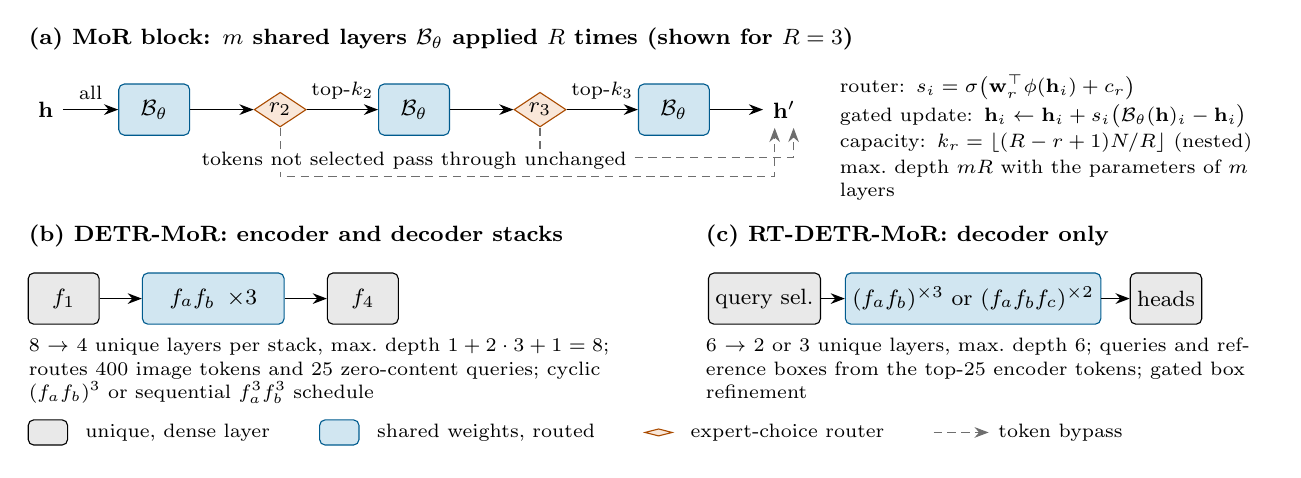
\begin{tikzpicture}[
  font=\figmed,
  blk/.style={draw, rounded corners=2pt, minimum height=6.5mm, minimum width=9mm, align=center, inner sep=2.5pt},
  uniq/.style={blk, fill=cGrey!15},
  shared/.style={blk, fill=cBlue!18, draw=cBlue!80!black},
  rt/.style={draw=cVerm!80!black, fill=cVerm!15, shape=diamond, aspect=1.5, inner sep=0.8pt, align=center},
  arr/.style={-{Stealth[length=1.8mm]}, semithick},
  skip/.style={-{Stealth[length=1.8mm]}, densely dashed, cGrey},
  lbl/.style={font=\figmed\bfseries, anchor=west, inner sep=0pt},
  note/.style={font=\figsmall, anchor=north west, align=left, inner sep=0pt},
]
% ---------------- (a) generic MoR block ----------------
\node[lbl] at (0,0.55) {(a) MoR block: $m$ shared layers $\mathcal{B}_\theta$ applied $R$ times (shown for $R=3$)};
\node[anchor=west] (in) at (0,-0.35) {$\mathbf{h}$};
\node[shared] (b1) at (1.6,-0.35) {$\mathcal{B}_\theta$};
\node[rt] (r2) at (3.2,-0.35) {$r_2$};
\node[shared] (b2) at (4.9,-0.35) {$\mathcal{B}_\theta$};
\node[rt] (r3) at (6.5,-0.35) {$r_3$};
\node[shared] (b3) at (8.2,-0.35) {$\mathcal{B}_\theta$};
\node (out) at (9.6,-0.35) {$\mathbf{h}'$};
\draw[arr] (in) -- node[above, font=\figsmall]{all} (b1);
\draw[arr] (b1) -- (r2);
\draw[arr] (r2) -- node[above, font=\figsmall]{top-$k_2$} (b2);
\draw[arr] (b2) -- (r3);
\draw[arr] (r3) -- node[above, font=\figsmall]{top-$k_3$} (b3);
\draw[arr] (b3) -- (out);
\draw[skip] (r2.south) -- ++(0,-0.62) -| ([xshift=-1.2mm]out.south);
\draw[skip] (r3.south) -- ++(0,-0.38) -| ([xshift=1.2mm]out.south);
\node[font=\figsmall, fill=white, inner sep=1pt] at (4.9,-1.0) {tokens not selected pass through unchanged};
\node[note, text width=55mm] at (10.3,0.1) {router: $s_i=\sigma\big(\mathbf{w}_r^{\top}\phi(\mathbf{h}_i)+c_r\big)$\\[1pt]
 gated update: $\mathbf{h}_i\leftarrow\mathbf{h}_i+s_i\big(\mathcal{B}_\theta(\mathbf{h})_i-\mathbf{h}_i\big)$\\[1pt]
 capacity: $k_r=\lfloor (R-r+1)N/R\rfloor$ (nested)\\[1pt]
 max.\ depth $mR$ with the parameters of $m$ layers};
% ---------------- (b) DETR-MoR ----------------
\node[lbl] at (0,-1.95) {(b) DETR-MoR: encoder and decoder stacks};
\node[uniq] (u1) at (0.45,-2.75) {$f_1$};
\node[shared, minimum width=18mm] (s1) at (2.35,-2.75) {$f_a f_b$ \,$\times 3$};
\node[uniq] (u4) at (4.25,-2.75) {$f_4$};
\draw[arr] (u1) -- (s1); \draw[arr] (s1) -- (u4);
\node[note, text width=78mm] at (0,-3.25) {8 $\to$ 4 unique layers per stack, max.\ depth \mbox{$1+2\cdot3+1=8$}; routes 400 image tokens and 25 zero-content queries; cyclic $(f_a f_b)^3$ or sequential $f_a^3 f_b^3$ schedule};
% ---------------- (c) RT-DETR-MoR ----------------
\node[lbl] at (8.6,-1.95) {(c) RT-DETR-MoR: decoder only};
\node[uniq, minimum width=14mm] (qs) at (9.35,-2.75) {query sel.};
\node[shared, minimum width=27mm] (s2) at (12.0,-2.75) {$(f_a f_b)^{\times 3}$ or $(f_a f_b f_c)^{\times 2}$};
\node[uniq] (hd) at (14.45,-2.75) {heads};
\draw[arr] (qs) -- (s2); \draw[arr] (s2) -- (hd);
\node[note, text width=72mm] at (8.6,-3.25) {6 $\to$ 2 or 3 unique layers, max.\ depth 6; queries and reference boxes from the top-25 encoder tokens; gated box refinement};
% ---------------- legend ----------------
\node[uniq, minimum width=5mm, minimum height=3.2mm] (l1) at (0.25,-4.45) {};
\node[anchor=west, font=\figsmall] (t1) at (0.6,-4.45) {unique, dense layer};
\node[shared, minimum width=5mm, minimum height=3.2mm, right=5mm of t1] (l2) {};
\node[anchor=west, font=\figsmall, right=1mm of l2] (t2) {shared weights, routed};
\node[rt, minimum width=3.5mm, right=5mm of t2] (l3) {};
\node[anchor=west, font=\figsmall, right=1mm of l3] (t3) {expert-choice router};
\draw[skip] ($(t3.east)+(5mm,0)$) -- ++(7mm,0) node[right, font=\figsmall, text=black]{token bypass};
\end{tikzpicture}
\caption{Mixture-of-Recursions (MoR) in detection transformers. (a)~A block of $m$ shared layers is applied $R$ times. Before every repeated pass, an expert-choice router keeps the top-$k_r$ tokens, which receive a gated residual update, and the remaining tokens pass through unchanged. (b)~In DETR, the middle layers of both the encoder and the decoder are shared and routed, keeping the maximum effective depth of eight. (c)~In RT-DETR, the whole decoder is a recursive block applied to the queries produced by query selection, keeping the maximum effective depth of six}
\label{fig:schematic}
\end{figure*}


Detection transformers cast object detection as direct set prediction: a decoder refines a fixed set of object queries through a stack of attention layers, and a bipartite matching loss assigns each query to at most one object~\cite{carion2020detr}. Decoder depth is therefore a central design variable. Each layer re-estimates every query's class and box, and successive layers progressively correct earlier estimates~\cite{carion2020detr,zhu2021deformable}. Real-time variants such as RT-DETR~\cite{zhao2024rtdetr} expose the number of decoder layers as a speed--accuracy knob, and every additional layer adds its own set of weights.

Two families of techniques reduce the cost of Transformer depth. \emph{Parameter sharing} reuses one block several times, as in Universal Transformers~\cite{dehghani2019universal}, ALBERT~\cite{lan2020albert} and recursive Transformers~\cite{bae2025relaxed}. \emph{Adaptive computation} lets each token use only as much depth as it needs, through halting~\cite{graves2016act,banino2021pondernet}, early exits~\cite{teerapittayanon2016branchynet} or learned routing~\cite{raposo2024mod,zhou2022expertchoice}. Mixture-of-Recursions (MoR)~\cite{bae2025mor} combines the two. A shared stack of layers is applied recursively, and a lightweight router decides, token by token, how many recursions each token receives. MoR improved the accuracy--efficiency trade-off of language models at equal compute~\cite{bae2025mor}, and it has since been adapted to vision backbones~\cite{visionmor2026,morswin2026,morst2026,edgerecvit2026,softmor2026}.

Whether these benefits carry over to the encoder--decoder of a detection transformer is not obvious. Decoder tokens are not image patches but object queries, and each query must be refined into exactly one box or into ``no object''. A recursive block applies the \emph{same} transformation repeatedly. That suits an iterative-refinement process in which every step makes a small correction to a hypothesis that is already close to its target, a view formalized by equilibrium formulations of the decoder~\cite{bai2019deq,wang2023deqdet}. It is less clear that one shared transformation can also \emph{form} object hypotheses from uninformative starting points. Efficient DETR~\cite{yao2021efficient} found that the many decoder layers of DETR are needed mainly because its object queries are randomly initialized, and that a dense prior removes most of this need. Detectors with poor and with informed query initialization may therefore respond very differently to recursive depth.

This paper evaluates MoR blocks in the two regimes. DETR~\cite{carion2020detr} starts every decoder query from a zero content vector and a learned, input-independent positional embedding. RT-DETR~\cite{zhao2024rtdetr} selects its queries from the highest-scoring encoder tokens and attaches a reference box to each, which every decoder layer then refines. We insert MoR into both detectors, keep the backbone, data and training recipe of each family fixed, and match every MoR model to the \emph{maximum effective depth} of its dense baseline. Our contributions are as follows.
\begin{itemize}
\item We present a controlled evaluation of MoR blocks inside the encoder--decoder of detection transformers, rather than in the backbone, covering two detector families that represent the two query-initialization regimes, two parameter-sharing schedules and two block/recursion splits.
\item In RT-DETR, the two MoR decoders outperform the six-layer decoder of equal maximum depth by \val{a.rt23-rt6.ap} and \val{a.rt32-rt6.ap}~AP with \val{rt23.decred}\% and \val{rt32.decred}\% fewer decoder parameters at matched decoder FLOPs. The $2\x3$ decoder outperforms the two-layer decoder with the same unique parameters by \val{a.rt23-rt2.ap}~AP. The gains concentrate at strict IoU thresholds and hold for \val{win.rt23-rt6} of \val{nclasses} classes.
\item In DETR, MoR halves the transformer parameters but loses \val{a.cyc-detr.ap} (cyclic) and \val{a.seq-detr.ap} (sequential)~AP. Inference-time routing probes show that this deficit does not come from routing decisions: removing the routing altogether leaves it in place.
\item An analysis of what the routers allocate shows that recursion acts as refinement of well-initialized queries in RT-DETR but cannot repair poorly initialized queries in DETR. We distill this into practical guidelines.
\end{itemize}

%% ===================================================================
\section{Related work}\label{sec:related}

\begin{table*}[t]
\caption{Configurations compared. ``Max depth'' is the maximum effective depth of the decoder (and of the encoder for DETR). ``Avg.\ depth'' is the average number of layer applications per query (per encoder token for DETR) implied by the capacity schedule}
\label{tab:configs}
\centering
\tabsize
\begin{tabular}{@{}llccccc@{}}
\toprule
Model & Routed stacks & Unique layers & $m\times R$ & Max depth & Avg.\ depth & Decoder capacity\\
\midrule
\rttwo & -- & 2 & -- & 2 & 2 & --\\
\rtsix & -- & 6 & -- & 6 & 6 & --\\
\rtA & decoder & 2 & $2\x3$ & 6 & 3.92 & 25\textrightarrow16\textrightarrow8\\
\rtB & decoder & 3 & $3\x2$ & 6 & 4.44 & 25\textrightarrow12\\
\midrule
DETR & -- & 8 / 8 & -- & 8 & 8 / 8 & --\\
\dcyc & enc.\,+\,dec. & 4 / 4 & $1{+}2\x3{+}1$ & 8 & 6.00 / 5.92 & 25\textrightarrow16\textrightarrow8\\
\dseq & enc.\,+\,dec. & 4 / 4 & $1{+}2\x3{+}1$ & 8 & 5.50 / 5.40 & 25\textrightarrow20\textrightarrow\dots\textrightarrow4\\
\bottomrule
\end{tabular}
\end{table*}


\paragraph{Detection transformers and query initialization.}
DETR~\cite{carion2020detr} removed anchors and non-maximum suppression through Hungarian matching~\cite{kuhn1955hungarian} but converges slowly. Deformable DETR~\cite{zhu2021deformable} introduced sparse multi-scale deformable attention, iterative box refinement and a two-stage variant that initializes queries from encoder proposals. Later work made queries more informative: conditional spatial queries~\cite{meng2021conditional}, anchor boxes as queries~\cite{liu2022dab}, query denoising~\cite{li2022dn}, and mixed query selection~\cite{zhang2023dino}. Efficient DETR~\cite{yao2021efficient} traced DETR's need for many decoder layers to the random initialization of its object queries and reference points, and with a dense prior closed the gap between one and six decoder layers. RT-DETR~\cite{zhao2024rtdetr} combines an efficient hybrid encoder with IoU-aware query selection to reach real-time speed, and RT-DETRv2~\cite{lv2024rtdetrv2}, D-FINE~\cite{peng2025dfine} and DEIM~\cite{huang2025deim} refine its training.
\paragraph{Weight sharing and recursion.}
Universal Transformers~\cite{dehghani2019universal} and ALBERT~\cite{lan2020albert} share weights across depth, looped Transformers apply one block repeatedly~\cite{giannou2023looped}, and relaxed recursive Transformers relax strict tying with layer-wise low-rank adapters~\cite{bae2025relaxed}. In detection, RecursiveDet~\cite{zhao2023recursivedet} shares decoder parameters across the stages of region-based detectors, and DEQDet~\cite{wang2023deqdet} models the decoder as a fixed-point iteration of a weight-tied layer, following deep equilibrium models~\cite{bai2019deq}.

\paragraph{Adaptive computation and routing.}
Adaptive computation time~\cite{graves2016act}, PonderNet~\cite{banino2021pondernet} and early-exit networks~\cite{teerapittayanon2016branchynet} vary depth per input. Sparse mixtures of experts~\cite{shazeer2017moe,fedus2022switch} route tokens to experts, expert-choice routing~\cite{zhou2022expertchoice} lets each expert select a fixed number of tokens, and Mixture-of-Depths~\cite{raposo2024mod} uses that mechanism to let tokens skip whole blocks. In vision, DynamicViT~\cite{rao2021dynamicvit} and A-ViT~\cite{yin2022avit} prune or halt tokens. For DETR encoders, Sparse DETR~\cite{roh2022sparse}, Focus-DETR~\cite{zheng2023focus} and Salience DETR~\cite{hou2024salience} restrict computation to selected tokens, and Lite DETR~\cite{li2023lite} updates low-level tokens less often. For decoders, QR-DETR~\cite{senthivel2024qrdetr} routes queries through or around each layer, and Dual-R-DETR~\cite{route2025detr} routes query-to-query interactions in self-attention. None of these methods shares weights across depth.

\paragraph{Mixture-of-Recursions in vision.}
MoR~\cite{bae2025mor} combines a recursive Transformer with token-level routing and recursion-wise key--value caching. Vision-MoR~\cite{visionmor2026}, MoR--Swin~\cite{morswin2026}, MoR-ST~\cite{morst2026}, Edge-RecViT~\cite{edgerecvit2026} and soft MoR~\cite{softmor2026} apply recursion with adaptive depth inside image \emph{backbones}, and some of them report detection results with conventional heads. To our knowledge, no prior study places MoR inside the encoder--decoder of a detection transformer or relates its benefit to how the object queries are initialized. That is the gap this work addresses.

%% ===================================================================
\section{Method}\label{sec:method}

\subsection{Decoder preliminaries}
A detection-transformer decoder maps $N$ queries $\mathbf{Q}^{(0)}\in\mathbb{R}^{N\times d}$ through layers $f_1,\dots,f_L$, $\mathbf{Q}^{(\ell)}=f_\ell(\mathbf{Q}^{(\ell-1)},\mathbf{M})$. Each layer consists of query self-attention, cross-attention to the encoder memory $\mathbf{M}$, and a feed-forward network. Every layer output is decoded by class and box heads and supervised through Hungarian matching. The two detectors differ in $\mathbf{Q}^{(0)}$:
\begin{itemize}
\item In DETR~\cite{carion2020detr}, the content part of each query is zero and the positional part is a learned embedding that does not depend on the image. Boxes are predicted from scratch at every layer.
\item In RT-DETR~\cite{zhao2024rtdetr}, the $N$ encoder tokens with the highest class scores become the content queries, each with a reference box $\mathbf{b}^{(0)}$. Every layer predicts a correction, $\mathbf{b}^{(\ell)}=\sigma\big(\sigma^{-1}(\mathbf{b}^{(\ell-1)})+\Delta\mathbf{b}^{(\ell)}\big)$, and cross-attention is deformable~\cite{zhu2021deformable}.
\end{itemize}

\subsection{Mixture-of-Recursions block}\label{sec:mor}
A MoR block consists of $m$ unique layers $\mathcal{B}_\theta=(f_1,\dots,f_m)$ that are applied $R$ times with the same weights. Its maximum effective depth is therefore $mR$, while its parameter count is that of $m$ layers. Following the expert-choice variant of MoR~\cite{bae2025mor,zhou2022expertchoice}, every recursion $r\geq2$ has its own router, a single linear layer with sigmoid output:
\begin{equation}
s^{(r)}_i=\sigma\big(\mathbf{w}_r^{\top}\phi(\mathbf{h}_i)+c_r\big),
\label{eq:router}
\end{equation}
where $\phi$ is a LayerNorm in RT-DETR-MoR and the identity in DETR-MoR. The first recursion is dense. Recursion $r$ keeps the $k_r$ highest-scoring tokens of the previously active set,
\begin{equation}
\begin{aligned}
\mathcal{A}^{(r)}&=\operatorname{top}\text{-}k_r\big\{s^{(r)}_i: i\in\mathcal{A}^{(r-1)}\big\},\\
k_r&=\max\Big(1,\Big\lfloor \tfrac{R-r+1}{R}\,N\Big\rfloor\Big),
\end{aligned}
\label{eq:capacity}
\end{equation}
so the active set can only shrink, and $N$ queries give capacities $25\!\to\!16\!\to\!8$ for $R=3$ and $25\!\to\!12$ for $R=2$. Active tokens are updated by a gated residual and inactive tokens pass through unchanged:
\begin{equation}
\mathbf{h}_i\leftarrow
\begin{cases}
\mathbf{h}_i+s^{(r)}_i\big(\mathcal{B}_\theta(\mathbf{h})_i-\mathbf{h}_i\big), & i\in\mathcal{A}^{(r)},\\
\mathbf{h}_i, & \text{otherwise.}
\end{cases}
\label{eq:gate}
\end{equation}
Self-attention inside a routed recursion runs only among active tokens, and cross-attention always sees the full memory. Because the top-$k$ selection is not differentiable, the router is trained only through its gate~(\ref{eq:gate}). We add no auxiliary router loss, so routing is learned purely from the detection objective.

\subsection{Integration into the two detectors}\label{sec:integration}
Figure~\ref{fig:schematic} shows both integrations, and Table~\ref{tab:configs} summarizes the configurations.

\paragraph{DETR-MoR (encoder and decoder).}
Both stacks of the eight-layer DETR follow a middle-cycle layout. A unique first layer and a unique last layer process all tokens, and between them two shared layers are applied $R=3$ times under routing. The maximum effective depth is $1+2\cdot3+1=8$, equal to the baseline, with four unique layers per stack instead of eight. The encoder routes the 400 image tokens ($400\!\to\!266\!\to\!133$) and the decoder routes the 25 queries. We compare two sharing schedules:
\begin{itemize}
\item \emph{cyclic}: the order is $(f_a,f_b)\times3$, with one routing decision before each repeated pass;
\item \emph{sequential}: the order is $f_a,f_a,f_a,f_b,f_b,f_b$, with a decision before every application, giving five routers per stack and decoder capacities $25\!\to\!20\!\to\!16\!\to\!12\!\to\!8\!\to\!4$.
\end{itemize}

\paragraph{RT-DETR-MoR (decoder only).}
The backbone, hybrid encoder and query selection are unchanged. The decoder is a pure cycle of $m$ shared layers applied $R$ times, with $m\times R\in\{2\x3,3\x2\}$, so the maximum effective depth is six, equal to the six-layer baseline. The gate also scales the box correction, $\mathbf{b}_i\leftarrow\sigma\big(\sigma^{-1}(\mathbf{b}_i)+s^{(r)}_i\Delta\mathbf{b}_i\big)$, so a query that is barely selected is barely moved. Each recursion has its own classification head and is supervised, while the box heads are shared. Denoising queries~\cite{li2022dn} are never routed.

\subsection{Routing probes}\label{sec:probes}
To test whether the learned routing is responsible for a model's accuracy, we change the routing \emph{at inference only}, on checkpoints trained with routing, and re-evaluate.
\begin{itemize}
\item \emph{Full}: every token is kept at every recursion, which removes routing. The learned gates are still applied.
\item \emph{Random}: tokens are kept at random under the trained capacities.
\item \emph{Oracle}: decoder only. Queries that the Hungarian matcher assigns to ground-truth objects in the default pass get priority under the trained capacities.
\end{itemize}
The \emph{full} probe is out of distribution for a routed checkpoint. A rise in AP would therefore indict the router, whereas a drop would prove little.

%% ===================================================================
\section{Experimental setup}\label{sec:setup}

\begin{table*}[t]
\caption{RT-DETR family on VOC2007 test. Decoder parameters include the per-layer heads. GFLOPs are for one $640\times640$ image with 25 queries}
\label{tab:rtdetr}
\centering
\tabsize
\begin{tabular}{@{}lcccccccc@{}}
\toprule
 & \multicolumn{2}{c}{Params (M)} & \multicolumn{2}{c}{GFLOPs} & & & & \\
\cmidrule(lr){2-3}\cmidrule(lr){4-5}
Model & Decoder & Total & Decoder & Total & \AP & \APfifty & \APseventyfive & $\mathrm{AP}_{85}$\\
\midrule
\rttwo & \val{rt2.decparams} & \val{rt2.params} & \val{rt2.decgflops} & \val{rt2.gflops} & \val{rt2.ap} & \val{rt2.ap50} & \val{rt2.ap75} & \val{rt2.ap85}\\
\rtsix & \val{rt6.decparams} & \val{rt6.params} & \val{rt6.decgflops} & \val{rt6.gflops} & \val{rt6.ap} & \val{rt6.ap50} & \val{rt6.ap75} & \val{rt6.ap85}\\
\rtA & \val{rt23.decparams} & \val{rt23.params} & \val{rt23.decgflops} & \val{rt23.gflops} & \val{rt23.ap} & \textbf{\val{rt23.ap50}} & \val{rt23.ap75} & \val{rt23.ap85}\\
\rtB & \val{rt32.decparams} & \val{rt32.params} & \val{rt32.decgflops} & \val{rt32.gflops} & \textbf{\val{rt32.ap}} & \val{rt32.ap50} & \textbf{\val{rt32.ap75}} & \textbf{\val{rt32.ap85}}\\
\midrule
\multicolumn{5}{@{}l}{\rtA{} $-$ \rtsix} & \val{d.rt23-rt6.ap} & \val{d.rt23-rt6.ap50} & \val{d.rt23-rt6.ap75} & \val{d.rt23-rt6.ap85}\\
\multicolumn{5}{@{}l}{\rtB{} $-$ \rtsix} & \val{d.rt32-rt6.ap} & \val{d.rt32-rt6.ap50} & \val{d.rt32-rt6.ap75} & \val{d.rt32-rt6.ap85}\\
\multicolumn{5}{@{}l}{\rtA{} $-$ \rttwo{} (same unique parameters)} & \val{d.rt23-rt2.ap} & \val{d.rt23-rt2.ap50} & \val{d.rt23-rt2.ap75} & \val{d.rt23-rt2.ap85}\\
\bottomrule
\end{tabular}
\end{table*}

\begin{table*}[t]
\caption{DETR family on VOC2007 test. All three models share an identical training recipe. GFLOPs are for one $640\times640$ image}
\label{tab:detr}
\centering
\tabsize
\begin{tabular}{@{}lccccccc@{}}
\toprule
 & \multicolumn{2}{c}{Params (M)} & \multicolumn{2}{c}{GFLOPs} & & & \\
\cmidrule(lr){2-3}\cmidrule(lr){4-5}
Model & Transformer & Trainable & Transformer & Total & \AP & \APfifty & \APseventyfive\\
\midrule
DETR & \val{detr.tfparams} & \val{detr.trainable} & \val{detr.tfgflops} & \val{detr.gflops} & \textbf{\val{detr.ap}} & \textbf{\val{detr.ap50}} & \textbf{\val{detr.ap75}}\\
\dcyc & \val{cyc.tfparams} & \val{cyc.trainable} & \val{cyc.tfgflops} & \val{cyc.gflops} & \val{cyc.ap} & \val{cyc.ap50} & \val{cyc.ap75}\\
\dseq & \val{seq.tfparams} & \val{seq.trainable} & \val{seq.tfgflops} & \val{seq.gflops} & \val{seq.ap} & \val{seq.ap50} & \val{seq.ap75}\\
\midrule
\multicolumn{5}{@{}l}{\dcyc{} $-$ DETR} & \val{d.cyc-detr.ap} & \val{d.cyc-detr.ap50} & \val{d.cyc-detr.ap75}\\
\multicolumn{5}{@{}l}{\dseq{} $-$ DETR} & \val{d.seq-detr.ap} & \val{d.seq-detr.ap50} & \val{d.seq-detr.ap75}\\
\bottomrule
\end{tabular}
\end{table*}


\paragraph{Data.}
We use PASCAL VOC~\cite{everingham2010voc}.
\begin{itemize}
\item \emph{Training pool}: VOC2007 and VOC2012 trainval (16{,}551 images). Because every detector uses 25 queries, the 15 images with more than 25 annotated objects are removed.
\item \emph{Split}: the remaining 16{,}536 images are split at random (seed 1111) into 13{,}229 training images and 3{,}307 validation images. The validation images are used only to select the checkpoint with the lowest validation loss.
\item \emph{Test}: VOC2007 test (4{,}952 images), with the same filter applied, leaving 4{,}945 images.
\end{itemize}

\paragraph{Detectors and training.}
Both families use a ResNet-34~\cite{he2016resnet} initialized from ImageNet. Neither loads detection-pretrained weights, so every transformer, router and head is trained from scratch. Images are resized to $640\times640$. Training uses horizontal flips, zoom-out, IoU-constrained cropping and photometric distortion, and the seed is 1111.

\emph{DETR family.}
\begin{itemize}
\item Architecture: the backbone, including batch normalization, is frozen. Pre-norm Transformer with $d=256$, 8 heads, feed-forward width 2048, eight encoder and eight decoder layers, and 25 queries over the $20\times20$ feature map.
\item Loss: cross-entropy with background weight 0.1, plus $5\times$ L1 and $2\times$ generalized-IoU~\cite{rezatofighi2019giou} box losses at every decoder output.
\item Optimization: AdamW~\cite{loshchilov2019adamw}, learning rate $1.4\times10^{-4}$, weight decay $10^{-4}$, batch size 32, 300 epochs, with the learning rate reduced tenfold at epoch 200.
\item The three DETR-family models use \emph{identical} training settings.
\end{itemize}

\emph{RT-DETR family.}
\begin{itemize}
\item Architecture: frozen batch-norm statistics, with backbone learning rate $10^{-5}$. One AIFI layer on the stride-32 features, a CCFM fusion neck~\cite{zhao2024rtdetr}, top-25 query selection, and deformable cross-attention (8 heads, 3 levels, 4 points) with feed-forward width 1024.
\item Loss: 50 denoising queries~\cite{li2022dn}, varifocal loss~\cite{zhang2021varifocal} ($\alpha=0.75$, $\gamma=2$), plus $5\times$ L1 and $2\times$ generalized-IoU losses on every decoder output and on the query-selection output.
\item Optimization: AdamW, learning rate $10^{-4}$, weight decay $10^{-4}$, gradient clipping at 0.1, 72 epochs, with the learning rate reduced tenfold at epoch 60.
\item Batch size, set by the memory of a single 16\,GB GPU: 23 (2L), 25 (6L), 20 (MoR $2\x3$) and 22 (MoR $3\x2$).
\end{itemize}

\paragraph{Evaluation.}
We report average precision (AP) averaged over IoU thresholds $\{0.50,0.55,\dots,0.95\}$, together with \APfifty{} and \APseventyfive{}.
\begin{itemize}
\item Per-class AP uses all-point interpolation of the precision--recall curve.
\item Objects marked \emph{difficult} are excluded both from the recall denominator and from scoring.
\item No score threshold or non-maximum suppression is applied. DETR outputs one detection per query (25 per image), and RT-DETR keeps its top 100 query--class pairs.
\end{itemize}
The protocol is applied identically to all models, but it is not the COCO 101-point implementation, so absolute values should be compared only within this study.

\paragraph{Complexity.}
We report parameters and floating-point operations (FLOPs, two per multiply--accumulate) for a single $640\times640$ image. FLOPs are counted with PyTorch's operator counter, with attention products added analytically and RepVGG branches fused. MoR FLOPs are counted as executed under the trained capacity schedule. We do not report latency, because the routed implementations are not kernel-optimized and a latency comparison would mostly measure implementation overhead.

\paragraph{Use of generative AI.}
A large language model was used to help draft the text of this manuscript and the analysis scripts that compile its tables and figures from the stored evaluation outputs. The authors verified every number, statement and reference and take full responsibility for the content.

%% ===================================================================
\section{Results}\label{sec:results}

\begin{figure}[t]
\centering
\begin{tikzpicture}
\begin{groupplot}[
  group style={group size=1 by 2, vertical sep=12mm, xlabels at=edge bottom},
  width=\columnwidth, height=40mm,
  xlabel={IoU threshold}, xmin=0.48, xmax=0.97,
  xtick={0.5,0.6,0.7,0.8,0.9}, xticklabel style={/pgf/number format/fixed, /pgf/number format/precision=1},
  grid=major, grid style={gray!20},
  tick label style={font=\figsmall}, label style={font=\figmed},
  legend style={font=\figsmall, draw=none, at={(0.5,1.02)}, anchor=south, legend columns=-1,
    /tikz/every even column/.append style={column sep=2.5mm}},
  every axis plot/.append style={thick, mark size=1.8pt},
]
\nextgroupplot[ylabel={$\Delta$AP vs.\ \rtsix}, ymin=-2.1, ymax=2.7]
\addplot[cGrey, densely dotted, forget plot] coordinates {(0.48,0) (0.97,0)};
\addplot[cBlue, mark=*] table[x=iou, y=drt23] {\tblPerIoU};
\addplot[cVerm, mark=square*, dashed] table[x=iou, y=drt32] {\tblPerIoU};
\addplot[cGrey, mark=triangle*, dashdotted] table[x=iou, y=drt2] {\tblPerIoU};
\legend{MoR $2\x3$, MoR $3\x2$, 2L (dense)}
\node[anchor=north west, font=\figmed\bfseries] at (rel axis cs:0.015,0.97) {(a) RT-DETR};
\nextgroupplot[ylabel={$\Delta$AP vs.\ DETR}, ymin=-5.7, ymax=0.7]
\addplot[cGrey, densely dotted, forget plot] coordinates {(0.48,0) (0.97,0)};
\addplot[cGreen, mark=diamond*] table[x=iou, y=dcyc] {\tblPerIoU};
\addplot[cPurple, mark=pentagon*, dashed] table[x=iou, y=dseq] {\tblPerIoU};
\legend{MoR cyclic, MoR sequential}
\node[anchor=south east, font=\figmed\bfseries] at (rel axis cs:0.985,0.03) {(b) DETR};
\end{groupplot}
\end{tikzpicture}
\caption{AP difference to the dense baseline at each IoU threshold. (a)~In RT-DETR, the gains of MoR grow with localization strictness and peak at IoU 0.80--0.85. (b)~In DETR, the deficit of MoR is roughly uniform across thresholds, so it is not a localization effect}
\label{fig:periou}
\end{figure}


\begin{figure*}[t]
\centering
\begin{tikzpicture}
\begin{axis}[
  ybar, bar width=3pt, width=\textwidth, height=38mm,
  ylabel={$\Delta$AP vs.\ \rtsix}, ymin=-2, ymax=3.8,
  xtick=data, symbolic x coords={plane,bicycle,bird,boat,bottle,bus,car,cat,chair,cow,table,dog,horse,mbike,person,plant,sheep,sofa,train,tv},
  xticklabel style={rotate=45, anchor=north east, font=\figsmall}, tick label style={font=\figsmall}, label style={font=\figmed},
  enlarge x limits=0.03, ymajorgrids, grid style={gray!20},
  legend style={font=\figsmall, draw=none, at={(0.5,1.03)}, anchor=south, legend columns=-1,
    /tikz/every even column/.append style={column sep=3mm}},
]
\addplot[fill=cBlue!70, draw=cBlue!60!black] table[x=cls, y=drt23] {\tblPerClass};
\addplot[fill=cVerm!35, draw=cVerm!70!black, postaction={pattern=north east lines}] table[x=cls, y=drt32] {\tblPerClass};
\legend{MoR $2\x3$, MoR $3\x2$}
\end{axis}
\end{tikzpicture}
\caption{Per-class AP difference between the RT-DETR-MoR decoders and the six-layer decoder of equal maximum depth. Each configuration improves \val{win.rt23-rt6} of the \val{nclasses} classes}
\label{fig:perclass}
\end{figure*}


\subsection{RT-DETR: recursion improves accuracy at matched depth}\label{sec:res-rt}

Table~\ref{tab:rtdetr} reports the RT-DETR family.
\begin{itemize}
\item Both MoR decoders outperform the six-layer decoder of equal maximum depth: \rtA{} by \val{a.rt23-rt6.ap}~AP and \rtB{} by \val{a.rt32-rt6.ap}~AP.
\item They do so with \val{rt23.decred}\% and \val{rt32.decred}\% fewer decoder parameters, and the whole detector shrinks by \val{rt23.totred}\% and \val{rt32.totred}\%.
\item The cleanest comparison is with \rttwo{}, which has the same unique decoder parameters as \rtA{}. Applying those two layers three times instead of once adds \val{a.rt23-rt2.ap}~AP. Adding four unshared layers (\rtsix{}) adds only \val{a.rt6-rt2.ap}~AP.
\end{itemize}
In this regime, reusing a small decoder recursively was a better use of depth than stacking new layers.
%% Appears only once analysis/out/bootstrap.json exists (see README.md).
\hasval{ci.B}{A paired bootstrap over the test images (\val{ci.B} resamples) gives 95\% intervals of [\val{ci.rt23-rt6.ap.lo}, \val{ci.rt23-rt6.ap.hi}]~AP for \rtA{} vs.\ \rtsix{}, [\val{ci.rt32-rt6.ap.lo}, \val{ci.rt32-rt6.ap.hi}] for \rtB{} vs.\ \rtsix{}, and [\val{ci.rt23-rt2.ap.lo}, \val{ci.rt23-rt2.ap.hi}] for \rtA{} vs.\ \rttwo{}. These intervals reflect test-set sampling only, not training-seed variance.}{}

\paragraph{Where the gain comes from.}
Figure~\ref{fig:periou}a breaks the difference down by IoU threshold.
\begin{itemize}
\item The gain grows with localization strictness: \rtA{} improves on \rtsix{} by \val{d.rt23-rt6.midmin} to \val{d.rt23-rt6.midmax}~AP at IoU 0.70--0.85, and \rtB{} by \val{d.rt32-rt6.midmin} to \val{d.rt32-rt6.midmax}~AP.
\item At IoU 0.50 the two configurations differ from the baseline by only \val{d.rt23-rt6.ap50} and \val{d.rt32-rt6.ap50}.
\item At the extreme threshold of 0.95, both are slightly below it (\val{d.rt23-rt6.ap95}, \val{d.rt32-rt6.ap95}).
\end{itemize}
The recursive decoders therefore find essentially the same objects as the six-layer decoder but place their boxes more precisely. This fits the gated, shared box-refinement step of Section~\ref{sec:integration}. The improvement is also not confined to a few categories: both configurations beat \rtsix{} on \val{win.rt23-rt6} of the \val{nclasses} classes, and \rtA{} beats \rttwo{} on \val{win.rt23-rt2} (Fig.~\ref{fig:perclass}).

\paragraph{Compute.}
The decoder FLOPs of the MoR models (\val{rt23.decgflops} and \val{rt32.decgflops}~G) match those of \rtsix{} (\val{rt6.decgflops}~G), as intended by depth matching. Most of this cost is not query processing. \val{rt23.vprojgflops}~G of it is the value projection of the deformable attention over the 8{,}400 memory tokens, which is recomputed at every block application. Because the memory is fixed and the weights are shared, this projection is identical across recursions of the same block. Caching it once per unique block would reduce the MoR decoders to an estimated \val{rt23.cachedgflops} and \val{rt32.cachedgflops}~G. This is the detection analogue of MoR's recursion-wise key--value caching~\cite{bae2025mor}, which our implementation does not yet exploit.

\subsection{DETR: recursion does not compensate for poor initialization}\label{sec:res-detr}

Table~\ref{tab:detr} reports the DETR family.
\begin{itemize}
\item MoR halves the trainable parameters (\val{cyc.trainred}\% fewer) and reduces the transformer FLOPs by \val{cyc.tfgflopsred}\% (cyclic) and \val{seq.tfgflopsred}\% (sequential).
\item Accuracy falls by \val{a.cyc-detr.ap}~AP (cyclic) and \val{a.seq-detr.ap}~AP (sequential), and the drop is spread across classes: the cyclic model is worse on \val{loss.cyc-detr} of \val{nclasses} and the sequential model on all \val{loss.seq-detr}.
\item Unlike in RT-DETR, the deficit is nearly constant across IoU thresholds (Fig.~\ref{fig:periou}b). For the cyclic model it lies between \val{d.cyc-detr.iouminabs} and \val{d.cyc-detr.ioumaxabs}~AP at every threshold.
\end{itemize}
The flat deficit means that MoR loses objects and class confidence, not box precision. The schedule matters too: the sequential schedule makes five routing decisions and sends only 12 of 25 queries into its second shared layer, and it loses almost three times as much as the cyclic one.

\subsection{Is the router responsible?}\label{sec:res-probes}

A natural explanation for the DETR result is that routing decisions made on poorly initialized queries are unreliable. If so, the router would withhold depth from the queries that need it. Table~\ref{tab:probes} rules this out at inference time. On the first 1{,}000 test images (\val{probe.cyc.nobj} matched objects), no probe moves AP by more than \val{probe.maxabs.all} in any model.
\begin{itemize}
\item \emph{Removing routing does not help}: running every query and token at full depth changes the cyclic DETR-MoR by \val{probe.cyc.full}~AP, against a deficit of \val{a.cyc-detr.ap}. Removing it only in the encoder or only in the decoder gives \val{probe.cyc.fullencoder} and \val{probe.cyc.fulldecoder}.
\item \emph{Guaranteeing depth to matched queries does not help}: the oracle probe gives \val{probe.cyc.oracle}.
\item \emph{Random routing} changes AP by only \val{probe.cyc.random}, the largest effect of any probe.
\item The sequential model behaves the same way, and in RT-DETR-MoR all probes stay within \val{probe.rt32.maxabs}~AP.
\end{itemize}
In both families, \emph{which} queries recurse at inference is nearly irrelevant. The DETR deficit therefore lies in what the shared weights learned during training, not in the routing decisions made at inference.

\begin{table}[t]
\caption{Inference-time routing probes on checkpoints trained with routing (first 1{,}000 VOC2007 test images). AP under the trained routing, and its change under each probe; \emph{full} removes routing, and \emph{oracle} prioritizes the queries matched to ground truth}
\label{tab:probes}
\centering
\tabsize
\setlength{\tabcolsep}{3pt}
\begin{tabular}{@{}lcccc@{}}
\toprule
Model & AP & Full & Random & Oracle\\
\midrule
DETR-MoR, cyc. & \val{probe.cyc.default} & \val{probe.cyc.full} & \val{probe.cyc.random} & \val{probe.cyc.oracle}\\
DETR-MoR, seq. & \val{probe.seq.default} & \val{probe.seq.full} & \val{probe.seq.random} & \val{probe.seq.oracle}\\
RT-DETR-MoR, $2\x3$ & \val{probe.rt23.default} & \val{probe.rt23.full} & \val{probe.rt23.random} & \val{probe.rt23.oracle}\\
RT-DETR-MoR, $3\x2$ & \val{probe.rt32.default} & \val{probe.rt32.full} & \val{probe.rt32.random} & \val{probe.rt32.oracle}\\
\bottomrule
\end{tabular}
\end{table}

\subsection{What recursion is spent on}\label{sec:res-depth}

\dcyc{} and \rtA{} form a matched pair. Both apply two shared blocks three times, with decoder capacities \val{probe.cyc.capacity}. Figure~\ref{fig:depth} shows, for each matched query, the recursion after which it exited and the IoU of its final box.
\begin{itemize}
\item \emph{DETR-MoR.} The router is not arbitrary. Queries that recurse beyond the first pass come from crowded images (\val{depth.cyc.2.objs} and \val{depth.cyc.3.objs} objects on average, against \val{depth.cyc.1.objs}) and end with much lower IoU (\val{depth.cyc.2.iou} and \val{depth.cyc.3.iou}, against \val{depth.cyc.1.iou}). The router sends the hard queries deeper, but the extra recursions do not lift them to the quality of the queries that exit early.
\item \emph{RT-DETR-MoR.} Queries exiting after one or two recursions reach the same IoU (\val{depth.rt23.1.iou} and \val{depth.rt23.2.iou}), and only the \val{depth.rt23.3.share}\% that use all three are lower (\val{depth.rt23.3.iou}). The queries enter the decoder already close to their objects, and recursion polishes them, which is consistent with the strict-IoU gains of Fig.~\ref{fig:periou}a.
\end{itemize}

The encoder routers of DETR-MoR show a related pattern. The cyclic router keeps \val{fg.cyc.2.fg}\% of foreground tokens but only \val{fg.cyc.2.bg}\% of background tokens at its last stage, a \val{fg.cyc.2.ratio}\x{} preference for objects that it learned without any supervision. The sequential router is not object-aware: its foreground-to-background ratio is \val{fg.seq.min}--\val{fg.seq.max}. It is also the weaker model, which suggests that object-aware allocation of encoder recursion during training matters, even though forcing full depth at inference does not recover the loss.

\begin{figure}[t]
\centering
\begin{tikzpicture}
\begin{groupplot}[
  group style={group size=1 by 2, vertical sep=6mm, xlabels at=edge bottom, xticklabels at=edge bottom},
  width=\columnwidth, height=36mm,
  xlabel={Exit recursion (passes over the 2 shared blocks)},
  xtick={1,2,3}, xmin=0.5, xmax=3.5,
  tick label style={font=\figsmall}, label style={font=\figmed},
  legend style={font=\figsmall, draw=none, at={(0.5,1.03)}, anchor=south, legend columns=-1,
    /tikz/every even column/.append style={column sep=3mm}},
  grid=major, grid style={gray!20},
]
\nextgroupplot[ybar, bar width=7pt, ymin=0, ymax=85, ylabel={Share (\%)}]
\addplot[fill=cGreen!70, draw=cGreen!60!black] table[x=stage, y=cycshare] {\tblDepth};
\addplot[fill=cBlue!35, draw=cBlue!70!black, postaction={pattern=north east lines}] table[x=stage, y=rtshare] {\tblDepth};
\legend{DETR-MoR (cyclic), RT-DETR-MoR ($2\x3$)}
\node[anchor=north east, font=\figmed\bfseries] at (rel axis cs:0.985,0.95) {(a) share};
\nextgroupplot[ymin=0.5, ymax=0.9, ylabel={Mean IoU}, every axis plot/.append style={thick, mark size=2pt}]
\addplot[cGreen, mark=diamond*] table[x=stage, y=cyciou] {\tblDepth};
\addplot[cBlue, mark=*, dashed] table[x=stage, y=rtiou] {\tblDepth};
\node[anchor=south west, font=\figmed\bfseries] at (rel axis cs:0.02,0.04) {(b) box quality};
\end{groupplot}
\end{tikzpicture}
\caption{Matched pair with identical recursion structure ($2$ shared blocks $\times$ 3 recursions, capacity 25$\to$16$\to$8), on the first 1{,}000 test images. (a)~Share of matched queries by exit recursion. (b)~Mean IoU of their final boxes. DETR-MoR sends hard queries deeper but cannot repair them, whereas RT-DETR-MoR queries are already accurate and are refined}
\label{fig:depth}
\end{figure}

%% ===================================================================
\section{Discussion}\label{sec:discussion}

\paragraph{Why query initialization decides the outcome.}
A weight-tied recursion applies one mapping repeatedly. It is well suited to a process in which every step makes a small correction to an estimate that is already near its target, the setting in which decoders behave like fixed-point iterations~\cite{wang2023deqdet}.
\begin{itemize}
\item \emph{RT-DETR.} Query selection supplies exactly this setting: content features and reference boxes taken from the encoder. Our measurements show the signature of refinement. The gains are concentrated at strict IoU thresholds, the box quality barely depends on exit depth, and the routing decisions are almost interchangeable.
\item \emph{DETR.} The decoder starts from input-independent queries, so its early layers must form object hypotheses and suppress duplicates through self-attention before later layers can refine them. DETR's AP improves by several points from its first to its last decoder layer~\cite{carion2020detr}, and Efficient DETR traced the need for this depth to the random initialization of the queries~\cite{yao2021efficient}. Forcing one set of shared weights to perform both the formation and the refinement stages appears to cost accuracy across all IoU thresholds. Our probes indicate that no routing policy recovers this capacity: the bottleneck is what the shared weights can represent, not which queries receive them.
\end{itemize}
Query initialization is the explanation that our evidence supports best, but it is not the only difference between the two settings:
\begin{itemize}
\item DETR-MoR also routes encoder tokens, whereas RT-DETR-MoR routes only decoder queries;
\item DETR-MoR has \val{cyc.trainred}\% fewer trainable parameters than its baseline;
\item the DETR backbone is frozen.
\end{itemize}
The routing probes and the matched-pair analysis, which isolates the detector family under identical recursion structures, make the initialization account the most consistent one.

\paragraph{Practical guidelines.}
\begin{enumerate}
\item Use MoR in decoders whose queries are initialized from the image, through query selection, anchor priors or denoising. In our experiments it reduced decoder parameters and improved accuracy.
\item Prefer cyclic sharing with few routing decisions over sequential schedules that starve later shared layers.
\item Do not expect inference savings from a depth-matched recursive decoder unless the memory projections of shared blocks are cached.
\item In detectors with input-independent queries, keep the early layers unique or initialize the queries from the encoder before sharing depth. Improving the router alone is unlikely to help.
\end{enumerate}

\paragraph{Limitations.}
\begin{itemize}
\item \emph{Single seed.} Each configuration was trained once. Two independently trained MoR configurations agree in sign, per-class pattern and IoU profile, but seed variance is not quantified.
%% 47,664 vs 38,160 optimizer steps, from the training logs (not a generated result)
\item \emph{Training budgets.} Batch size varied with GPU memory, so \rtA{} received about 25\% more optimizer steps than \rtsix{}. In addition, both \rtsix{} and \rtA{} were still improving at the final epoch.
\item \emph{Benchmark and protocol.} All experiments use VOC at $640\times640$ with at most 25 objects per image and a custom all-point AP implementation.
\item \emph{Missing measurements and baselines.} We report FLOPs but no measured latency, and we did not train a parameter-matched four-layer DETR baseline.
\end{itemize}
Multi-seed runs, COCO-scale experiments, cached memory projections and latency measurements are the natural next steps.

%% ===================================================================
\section{Conclusion}\label{sec:conclusion}

We evaluated Mixture-of-Recursions blocks inside two detection transformers that differ in how their object queries are initialized. When queries come from encoder-based query selection, as in RT-DETR, a recursive decoder of two or three shared layers matches the maximum depth of a six-layer decoder and exceeds its accuracy with up to \val{rt23.decred}\% fewer decoder parameters, mainly by localizing objects more precisely. When queries start from input-independent embeddings, as in DETR, the same mechanism halves the transformer parameters but costs accuracy. That cost persists when routing is removed, randomized or oracle-guided at inference, which points to the shared weights, not the router, as the limiting factor. Recursive depth is therefore an effective way to compress detection decoders, provided that the queries it refines are well initialized.

\backmatter

\section*{Statements and Declarations}

\bmhead{Funding} Provided on the separate title page (double-blind review).

\bmhead{Competing interests} The authors declare that they have no competing interests.

\bmhead{Ethics approval and consent} Not applicable.

\bmhead{Data availability} PASCAL VOC is publicly available (\url{http://host.robots.ox.ac.uk/pascal/VOC/}). The evaluation outputs supporting the findings are available from the corresponding author on reasonable request.

\bmhead{Code availability} Code and configurations will be released upon acceptance. They are withheld during review for anonymity.

\bmhead{Author contributions} Provided on the separate title page.

\bibliography{references}

\end{document}
